\documentclass{article} % For LaTeX2e
\usepackage{nips2015,times}
\usepackage{hyperref}
\usepackage{url}
\usepackage{graphicx}
\graphicspath{ {../assets/} }
\usepackage{biblatex}
\addbibresource{refs.bib}


\title{CSE 546 Assignment 1 -- Part 1: Environments}


\author{
   Mohammed Nasheed Yasin \\
   Department of Linguistics\\
   University at Buffalo, SUNY\\
   Buffalo, NY 14260 \\
   \texttt{m44@buffalo.edu}
}

% The \author macro works with any number of authors. There are two commands
% used to separate the names and addresses of multiple authors: \And and \AND.
%
% Using \And between authors leaves it to \LaTeX{} to determine where to break
% the lines. Using \AND forces a linebreak at that point. So, if \LaTeX{}
% puts 3 of 4 authors names on the first line, and the last on the second
% line, try using \AND instead of \And before the third author name.

\newcommand{\fix}{\marginpar{FIX}}
\newcommand{\new}{\marginpar{NEW}}

\nipsfinalcopy

\begin{document}


\maketitle

\begin{abstract}
    This report explains my experiments with environments in RL.
    It focuses on the differences between stochastic and deterministic environments,
    and introduces commonly used rendering methodologies.
\end{abstract}

\section{The Environments}

There are certain features that are common to both the stocastic and deterministic environments.

\subsection*{Environmental Elements}
\begin{figure}[h]
    \begin{center}
        
\includegraphics[scale=0.50]{elements.png}
    \end{center}
    \caption{Environmental elements (from left to right; top to bottom) Agent, Goal,
        Negative Reward, Reward}
\end{figure}

\begin{enumerate}
    \item The enivironment is a \verb|6x6| grid. With \verb|36| possible states. The goal is
        to reach the oasis shown in picture 1 with the maximal reward within a 
        (configurable) number of time steps.
    \item The agent randomly (uniformly) takes one of four possible actions:
    \begin{itemize}
        \item Left
        \item Right
        \item Up
        \item Down
    \end{itemize}
    \item The reward space is continous with values ranging from -0.5 to 0.5. The terminal/goal state
        has a reward of 1 and the initial state has a reward of 0.
    \item Every state has a reward associated to it and the size of the 
        cactus/lemonade is indicative of the reward.
    \item Landing on a square causes the reward on that square to be consumed.
        i.e. landing on the same square again will yield no reward (0 reward).
    \item The rewards and negative rewards are spread randomly accross the grid on
        initialization.
    \item Resetting the environment will not change the location or distribution of the rewards
        and goal state. It only alters the initial state of the agent.
\end{enumerate}

\begin{figure}[h]
    \begin{center}
        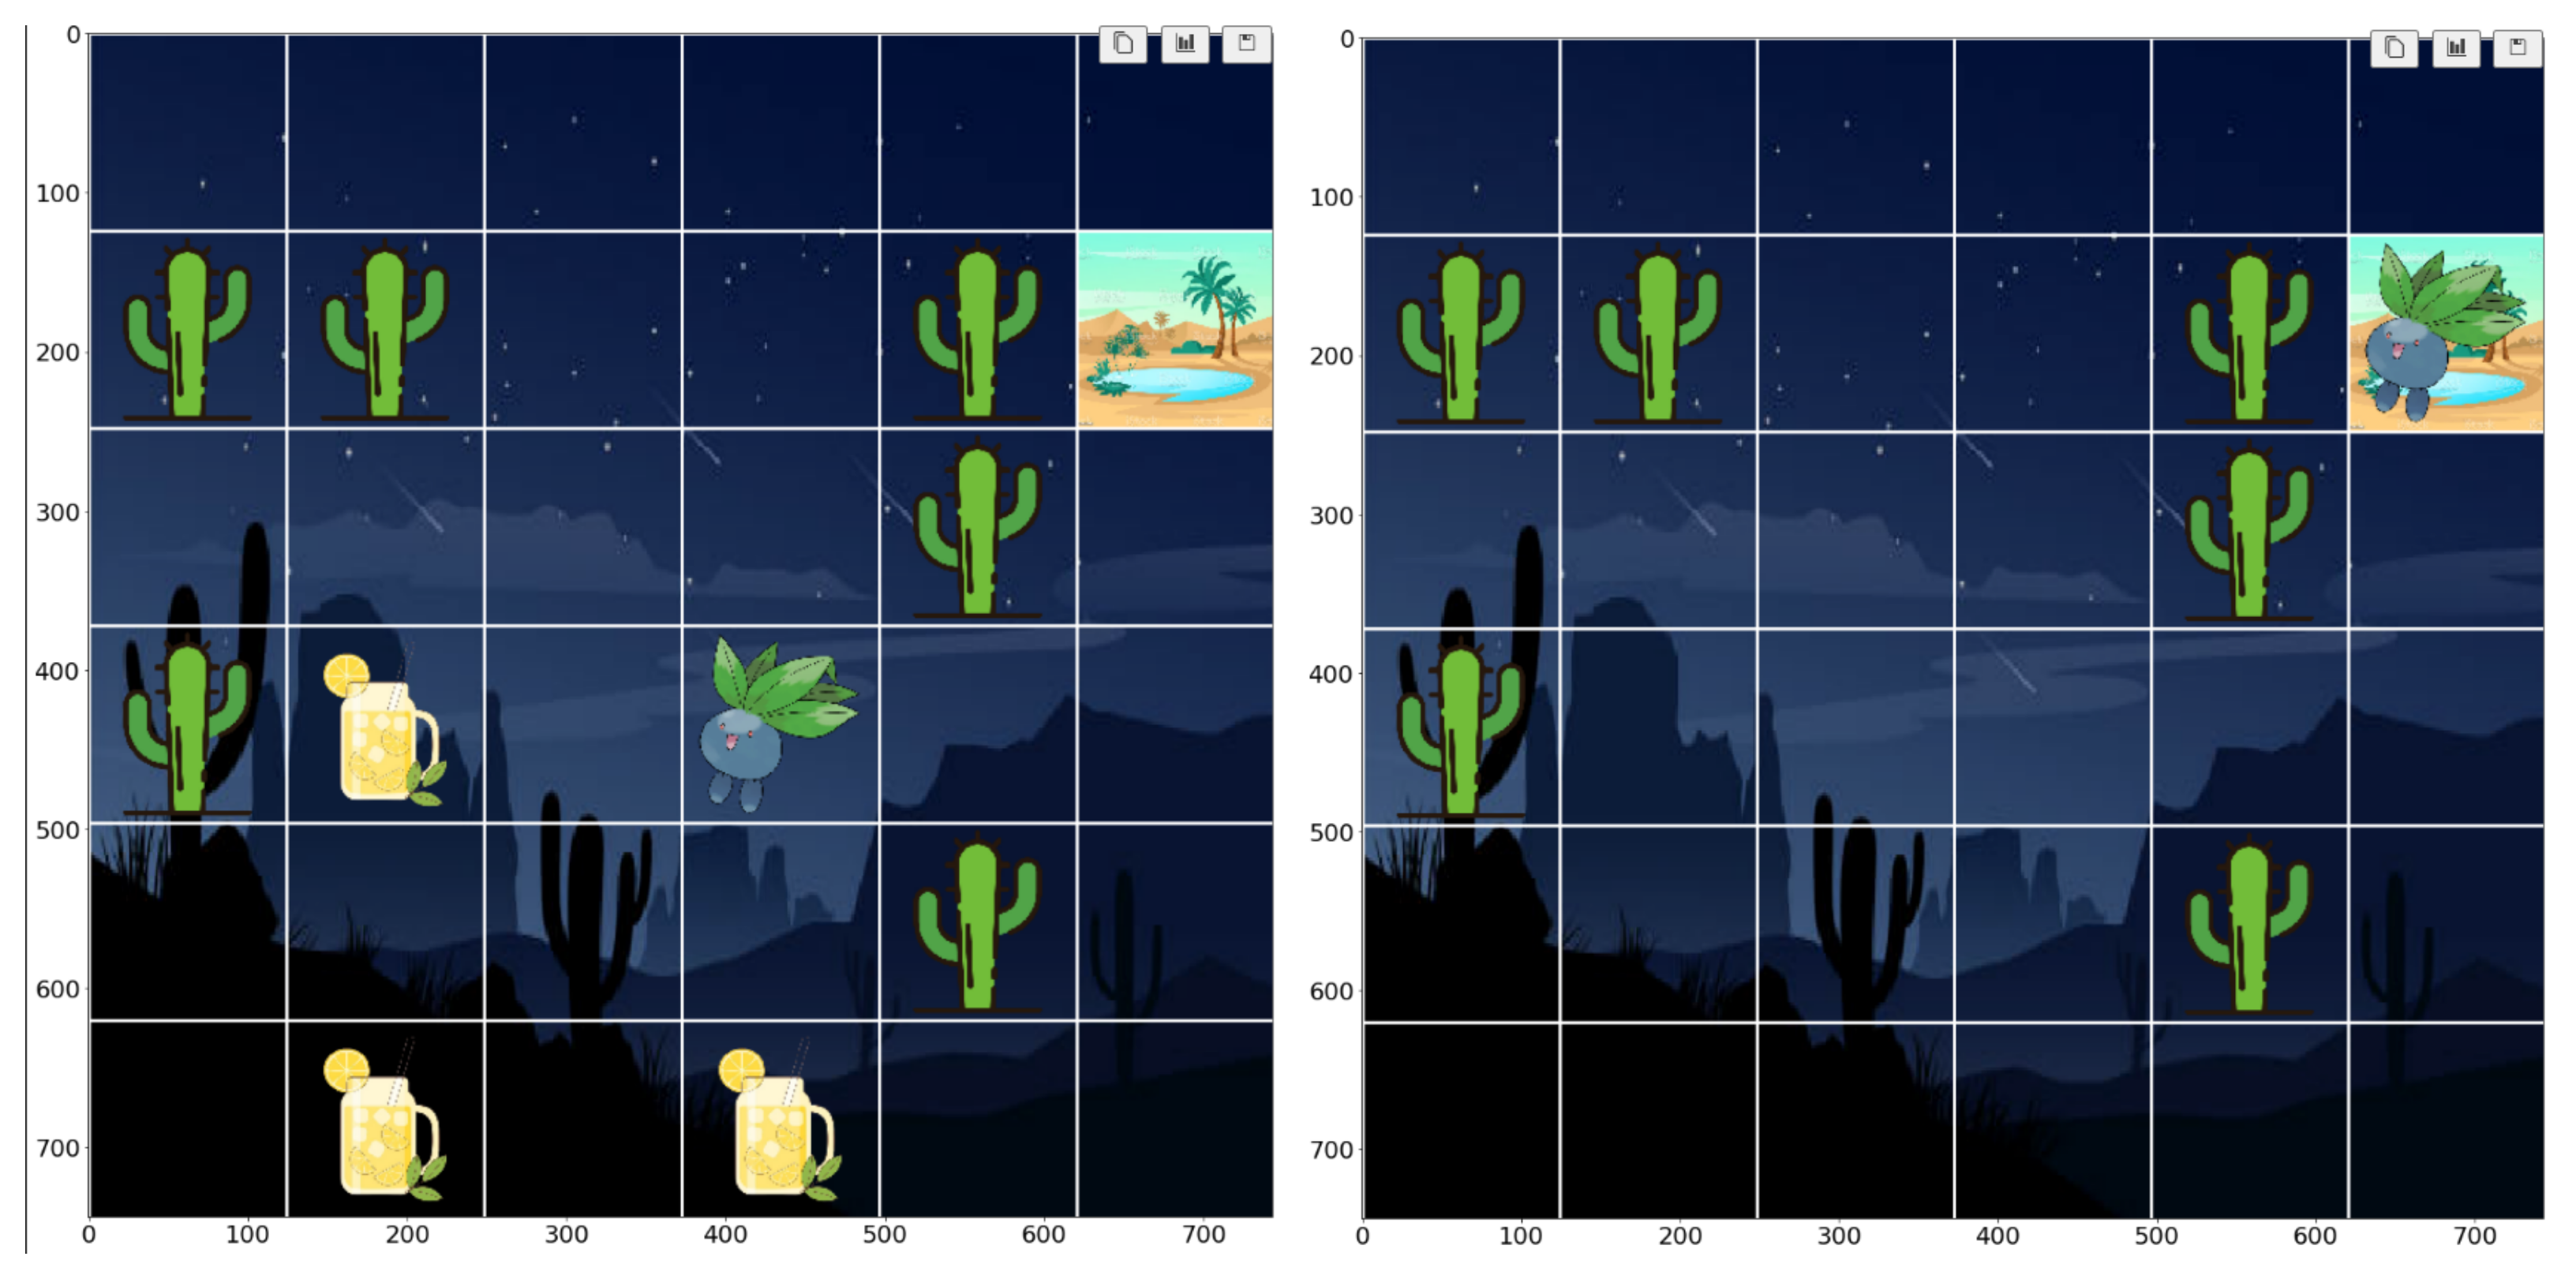
\includegraphics[scale=0.50]{vis.png}
    \end{center}
    \caption{Environment visualizations accross two seperate episodes}
\end{figure}



\subsection{Stocasticity}
An enviroment is called stocastic when the result of an action (i.e. its success or its 
reward) is not guaranteed. Formally, given the same state $s_0$ and action $a$ the next state
$s_1$ and reward $r$ will be probability distributions.

In the \verb|GridEnviroment| defined in this report, stocasticity stems is the stocasticity
can be described as follows:
\begin{itemize}
    \item For every action there is a $2/3^{rd}$ chance that the action is performed as
        expected (\verb|as-is|), a $2/9^{th}$ chance that it is the \verb|double| of what 
        is expected and a $1/9^{th}$ chance of it being a \verb|mirror| action.
    \item The reward (and negative reward) for each state is distributed in a reciprocal
        fashion. i.e. $1/9^{th}$ the reward for coming through the \verb|as-is| action,
        $2/9^{th}$ reward when coming via the \verb|double| action and $2/3^{rd}$ reward when
        coming via a \verb|mirror| action.
    \item For instance on a 5x5 grid where the reward on each square is 1 (for simplicity):
    \newline
    If $s_0$ \verb|=(2,3)| and $a$ \verb|= RIGHT|:
        \begin{itemize}
            \item $2/3^{rd}$ chance $s_1$ \verb|=(2,4)| and $r$ \verb|=1/9|
            \item $2/9^{th}$ chance $s_1$ \verb|=(2,5)| and $r$ \verb|=2/9|
            \item $1/9^{th}$ chance $s_1$ \verb|=(3,2)| and $r$ \verb|=2/3|
        \end{itemize}
    \item Exception: Landing on the \verb|goal| state will always yield a maximal reward
        (of 1 for the above example) regardless of how the agent got there.
\end{itemize}

\subsection{Safety in AI}
The following are properties of the environment that ensure valid behavior from the agent:

\begin{enumerate}
    \item The environment was created using Open AI's Gym library \cite[]{1606.01540}
        which ensures the minimum best practices in env definition are met through useful
        APIs like \verb|check_env| and an in-built Pseudo-random number generator (PRNG).
    \item The PRNG referenced above is seeded with a hard-coded number in order to ensure
        \textit{execution replicability} accross devices.
    \item The action space, reward space, action mode space, goal and initial agent position
        are defined using Gym's spaces API. All were initialized in a way that the use the same
        PRNG which ensures end to end replicability.
    \item The result of any action (left, right, top, down) are clipped to the min and max
        values of 0 and \verb|GridSize| (6 in our case) respectively, ensuring that the
        agent never leaves the environment.
    \item The reward of all states is consumed once the agent lands in that state, preventing 
        the agent from settling down in a \textit{high-reward} neighborhood.
    \item The reward at the goal$\backslash$target is 50\% higher than the highest possible reward for
        any non terminal state, which helps the agent prioritize the true objective.
    \item The stocasticity of the starting point and limited time steps will nudge the agent
        to build strategies that accumulate the maximal reward in the shortest time.
\end{enumerate}

\subsection*{Code Base}
The code for this assignment has been uploaded to \url{https://github.com/nasheedyasin/cse546-rl-assignments}

\begin{figure}[h]
    \begin{center}
        \includegraphics[scale=0.395]{commits.png}
    \end{center}
    \caption{Commit history.}
\end{figure}

\printbibliography

\end{document}